\documentclass[aspectratio=169, table]{beamer}
\usepackage[utf8]{inputenc}
\usepackage{xcolor}

\usepackage{multicol}
\usepackage{booktabs}
\usepackage{arydshln}
\usepackage[abs]{overpic}
\usepackage{tikz}
\usetikzlibrary{fadings}
%\usepackage{enumitem}
%\usepackage[table]{xcolor} 

\usepackage{empheq}

\definecolor{redp}{RGB}{245,86,91}
\definecolor{greenp}{rgb}{0.0, 0.51, 0.5}
\definecolor{yellowp}{rgb}{0.59, 0.44, 0.09}
\definecolor{greencol}{rgb}{0.0,0.4,0.0}
\definecolor{fcolor}{rgb}{0.8, 0.4, 0.0}
\definecolor{bluep}{rgb}{205,219,194}
\definecolor{greenp}{RGB}{73,165,150}

\newcommand{\enb}[1]{\textcolor{poliblue1}{\textbf{#1}}}
\newcommand{\eno}[1]{\textcolor{orangep}{\textbf{#1}}}
\definecolor{softblue}{cmyk}{.2, .1, .1, .2}
\newcommand{\soft}[1]{\textcolor{softblue}{#1}}

\title{Optimistic Policy Optimization via Multiple Importance Sampling}
\date[AAA]{\vspace{0.2cm} \\ \small{ 19th September 2019 \\ Markets, Algorithms, Prediction and Learning Workshop, Politecnico di Milano, Milano, Italy}}
\author[M. Papini]{\textbf{Matteo Papini} \quad Alberto Maria Metelli\\
						{Lorenzo Lupo \quad Marcello Restelli}}

\usetheme{polimithx}
\usetikzlibrary{calc}

\usepackage[customcolors,shade]{hf-tikz}

%%%%%%%%%%%%%%%%%%%%%%%%%% BIBLIOGRAPHY
\usepackage{natbib}
\bibliographystyle{apalike}
% make bibliography entries smaller
\renewcommand\bibfont{\scriptsize}
% If you have more than one page of references, you want to tell beamer
% to put the continuation section label from the second slide onwards
\setbeamertemplate{frametitle continuation}[from second]

%CUSTOM COMMANDS

\usepackage[many]{tcolorbox}
\usetikzlibrary{decorations.pathreplacing}
\usetikzlibrary{arrows,shapes}
\usetikzlibrary{positioning}

\usepackage{mymacros}

\begin{document}

\setbeamertemplate{caption}{\raggedright\insertcaption\par}

\begin{frame}[noframenumbering]
\titlepage
\end{frame}

\begin{frame}
\frametitle{Reinforcement Learning~\citep{sutton2018reinforcement}} 
\begin{center}
	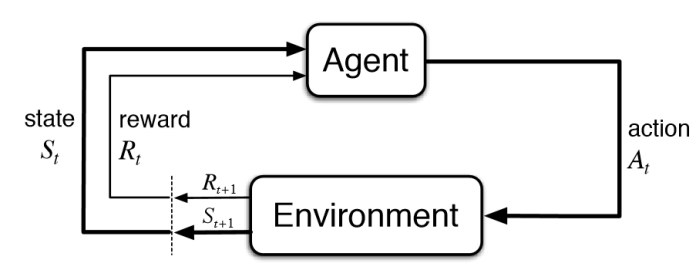
\includegraphics[width=.65\linewidth]{rl.jpg}
\end{center}
		\begin{itemize}
			\setlength{\itemsep}{8pt}
			\item<2-> Policy $\pi:\Sspace\to\Delta(\Aspace)$
			\item<3-> Trajectories $\tau = (s_0, a_0, r_1, s_1,\dots)$
			\item<4-> Return $R(\tau) = \sum_{t=0}^{T-1}\gamma^t r_{t+1}$
			\item<5-> Goal: $\max\limits_{\pi} \mathbb{E}_{\pi}\left[R(\tau)\right]$
		\end{itemize}
\end{frame}

\begin{frame}
\frametitle{Exploration vs Exploitation}
\centering
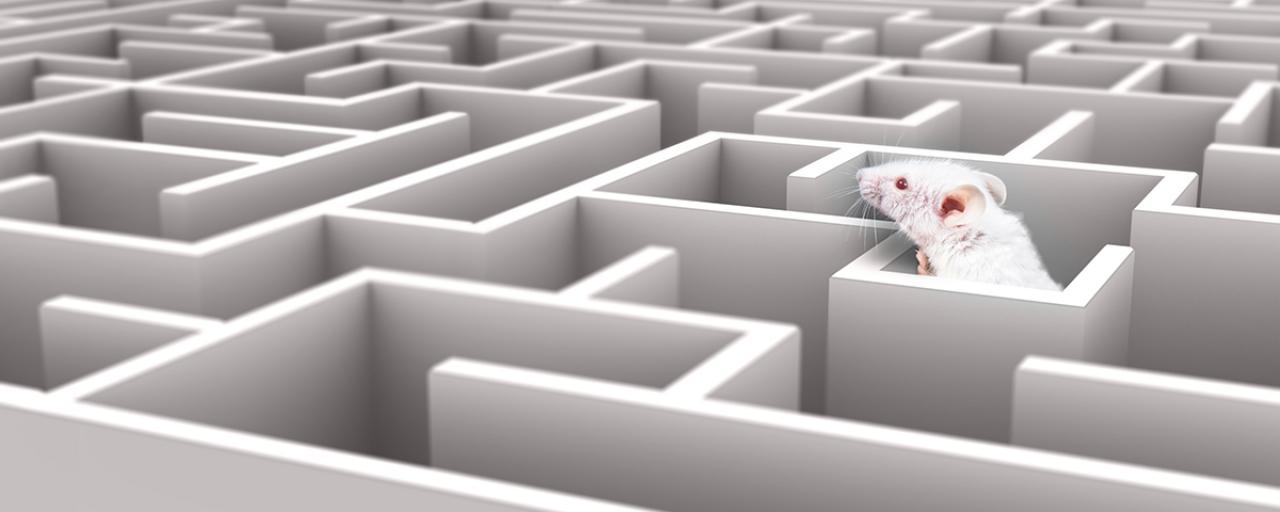
\includegraphics[width=\textwidth]{mouse.jpg}
\end{frame}

\begin{frame}
\frametitle{Continuous Reinforcement Learning}
\begin{columns}
		\begin{column}{.5\textwidth}
			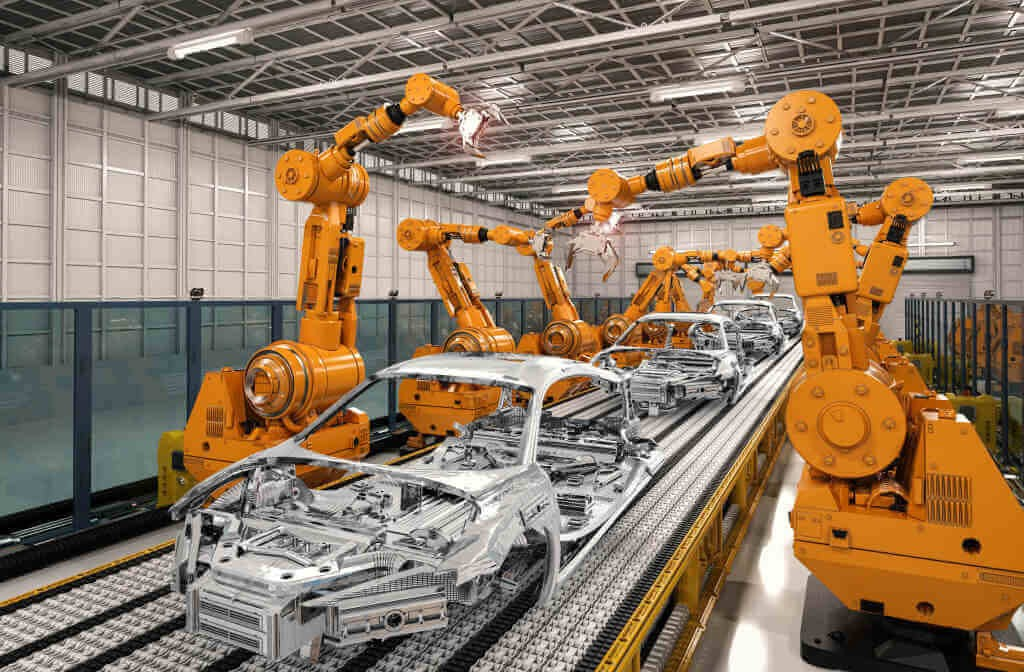
\includegraphics[width=\textwidth]{robots.jpeg}
		\end{column}
	\hfill
			\begin{column}{.5\textwidth}
			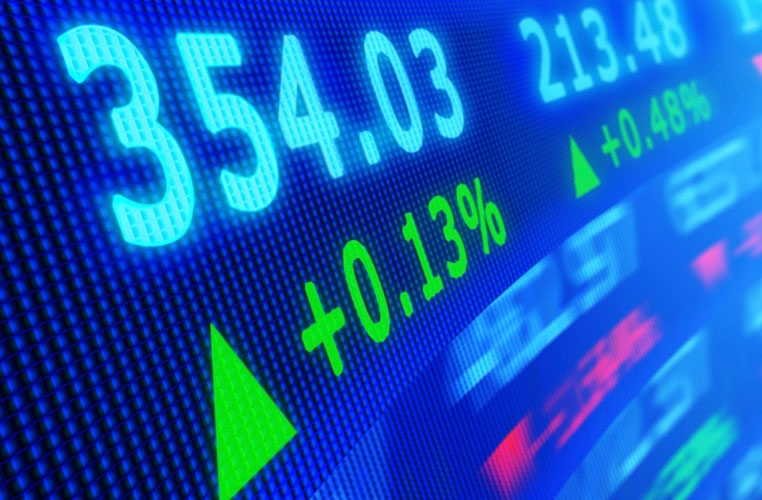
\includegraphics[width=\textwidth]{finance.jpg}
		\end{column}
\end{columns}
\end{frame}

\begin{frame}
\frametitle{Policy Optimization} 
\begin{columns}
\begin{column}{.65\textwidth}
\begin{overlayarea}{\textwidth}{\textheight}
\begin{itemize}
	\setlength{\itemsep}{25pt}
	\item \enb{Parameter space} $\Theta \subseteq \Reals^d$
	\item<2-> A \enb{parametric policy} $\pi_{\vtheta}$ for each $\vtheta\in\Theta$
	\item<3-> Each inducing a distribution $p_{\vtheta}$ over \enb{trajectories}
	\item<4-> A \enb{return} $R(\tau)$ for every trajectory $\tau$
	\item<5-> {Goal: $\max\limits_{\vtheta\in\Theta} J(\vtheta) = \Exp_{\tau\sim p_{\vtheta}}\left[R(\tau)\right]$}
\end{itemize}
\end{overlayarea}
\end{column}
\begin{column}{.35\textwidth}
\begin{overlayarea}{\textwidth}{\textheight}
	\only{
	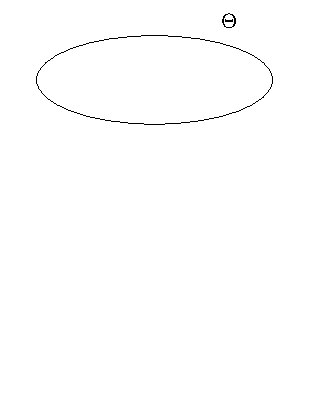
\includegraphics[]{animation/spaces1.pdf}}<1>
	\only{
	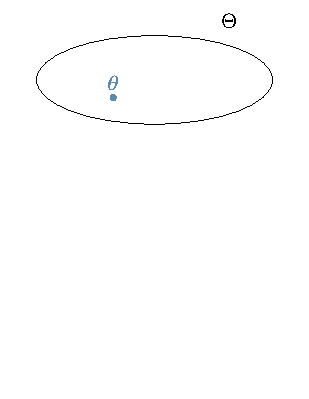
\includegraphics[]{animation/spaces2.pdf}}<2>
	\only{
	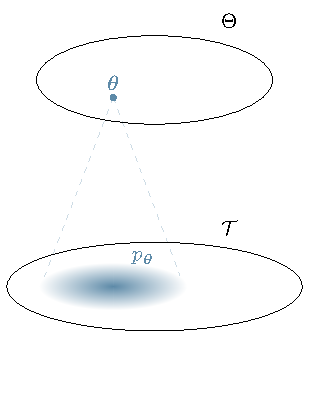
\includegraphics[]{animation/spaces3.pdf}}<3>
	\only{
	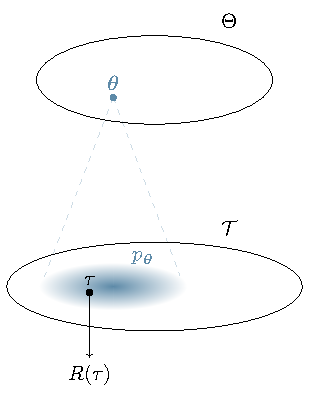
\includegraphics[]{animation/spaces4.pdf}}<4>
	\only{
	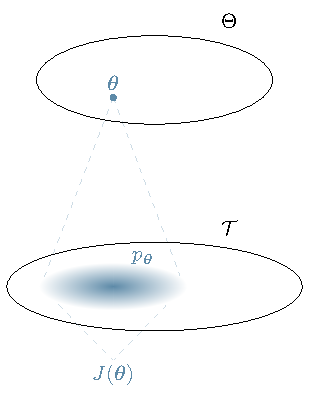
\includegraphics[]{animation/spaces5.pdf}}<5>
\end{overlayarea}
\end{column}
\end{columns}
\end{frame}

\begin{frame}
\frametitle{Policy Gradient Methods}
\begin{overlayarea}{\textwidth}{\textheight}
\begin{itemize}
	\setlength{\itemsep}{15pt}
	\item<1-> \enb{Gradient ascent} on $J(\vtheta)$
	\item<2-> Popular algorithms: {\bf REINFORCE}~\citep{williams1992simple},
	{\bf PGPE}~\citep{sehnke2008policy},
	{\bf TRPO}~\citep{schulman2015trust}, {\bf PPO}~\citep{schulman2017proximal}
\end{itemize}
\vspace{15pt}
\only<3->{
\begin{columns}
	\begin{column}{.5\textwidth}
		\centering
		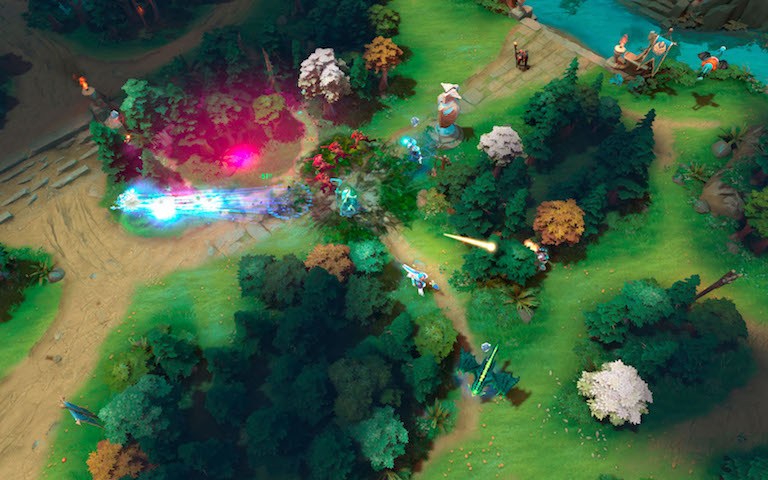
\includegraphics[width=.8\textwidth]{dota.jpg}
		\\
		\emph{Dota 2~\citep{OpenAI_dota}}
	\end{column}
	\begin{column}{.5\textwidth}
		\centering
		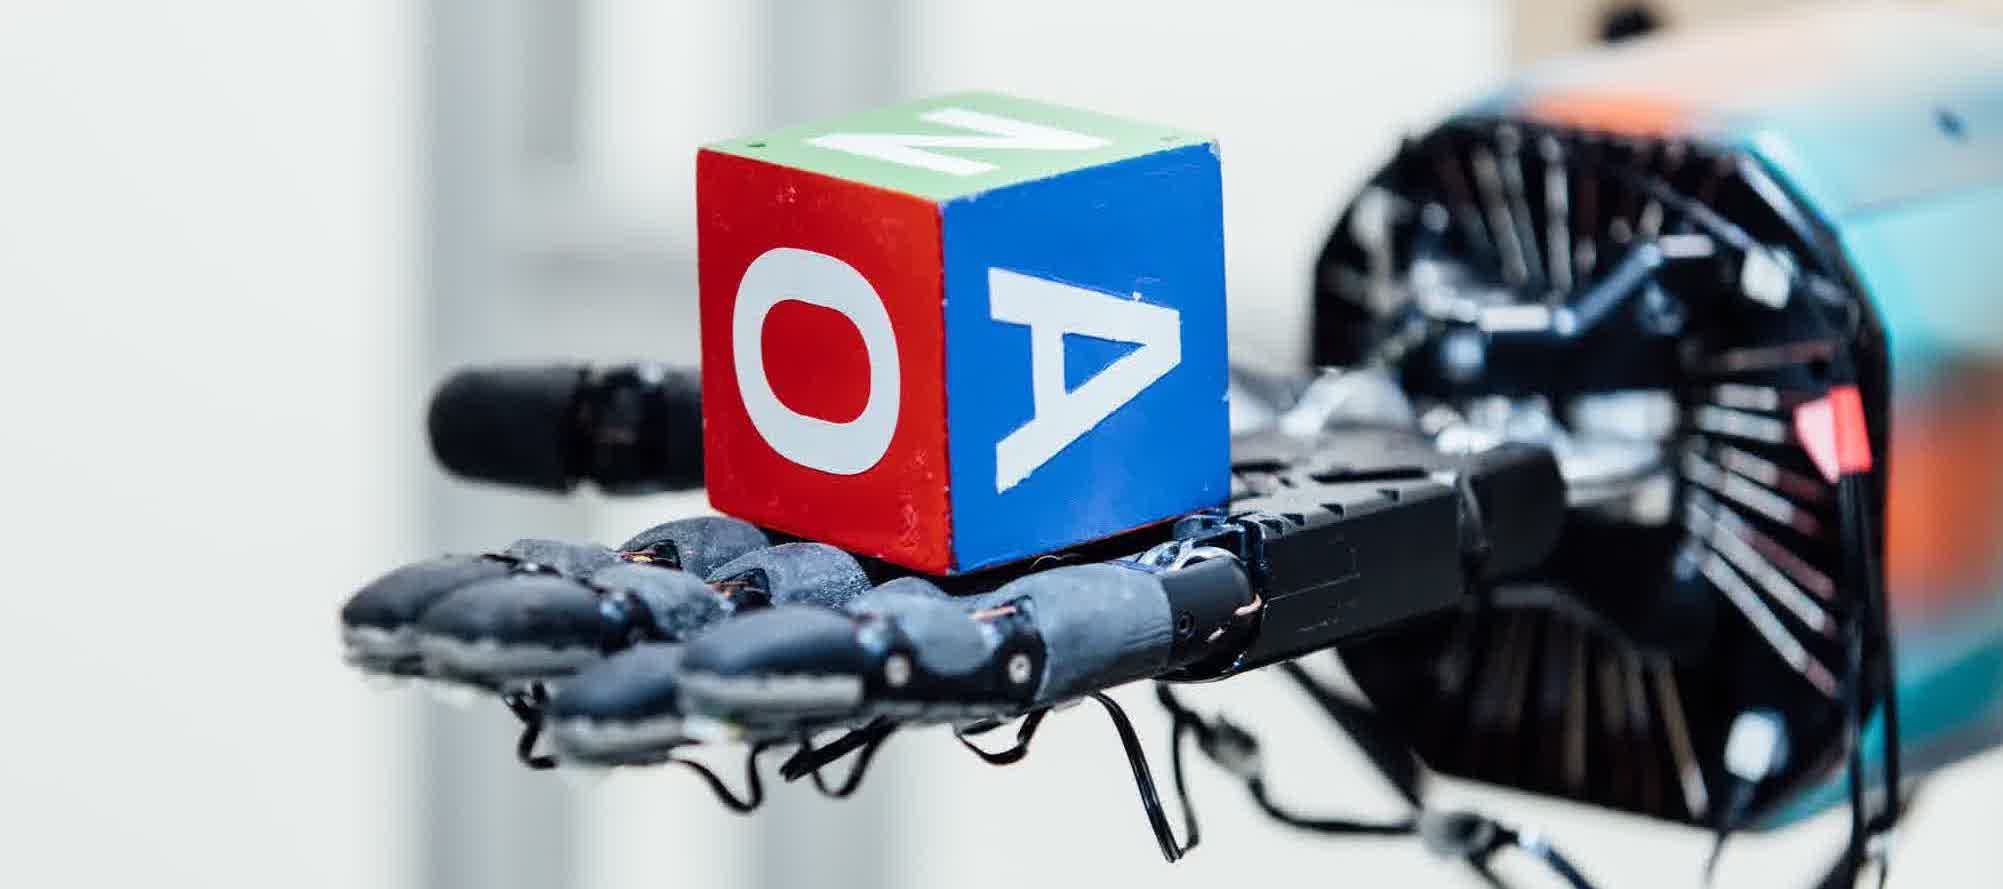
\includegraphics[width=.8\textwidth]{hand.jpg}
		\\ 
		\emph{Manipulation ~\citep{andrychowicz2018learning}}
	\end{column}
\end{columns}
}
\end{overlayarea}
\end{frame}

\begin{frame} 
\frametitle{Exploration in Policy Optimization}
\begin{columns}
\begin{column}{.65\textwidth}
\begin{overlayarea}{\textwidth}{\textheight}
\vspace{.5cm}
\begin{itemize}
	\setlength{\itemsep}{20pt}
	\item<1-> Policy Gradient fails with \eno{sparse rewards}~\citep{kakade2002approximately}
	\item <2-> Non-convex objective $\implies$ \eno{local minima}
	\end{itemize}
	\vspace{1cm}	
	\only<3->{
	\enb{Entropy bonus}~\citep{haarnoja2018soft}:
	\vspace{10pt}
	\begin{itemize}
		\setlength{\itemsep}{8pt}
		\item<4-> \emph{Undirected}
		\item<5-> \eno{Unsafe}
		\item<6-> Little theoretical understanding~\citep{ahmed2018understanding}
	\end{itemize}
}
\end{overlayarea}
\end{column}
\begin{column}{.35\textwidth}
\begin{overlayarea}{\textwidth}{\textheight}
\vspace{.2\textheight}
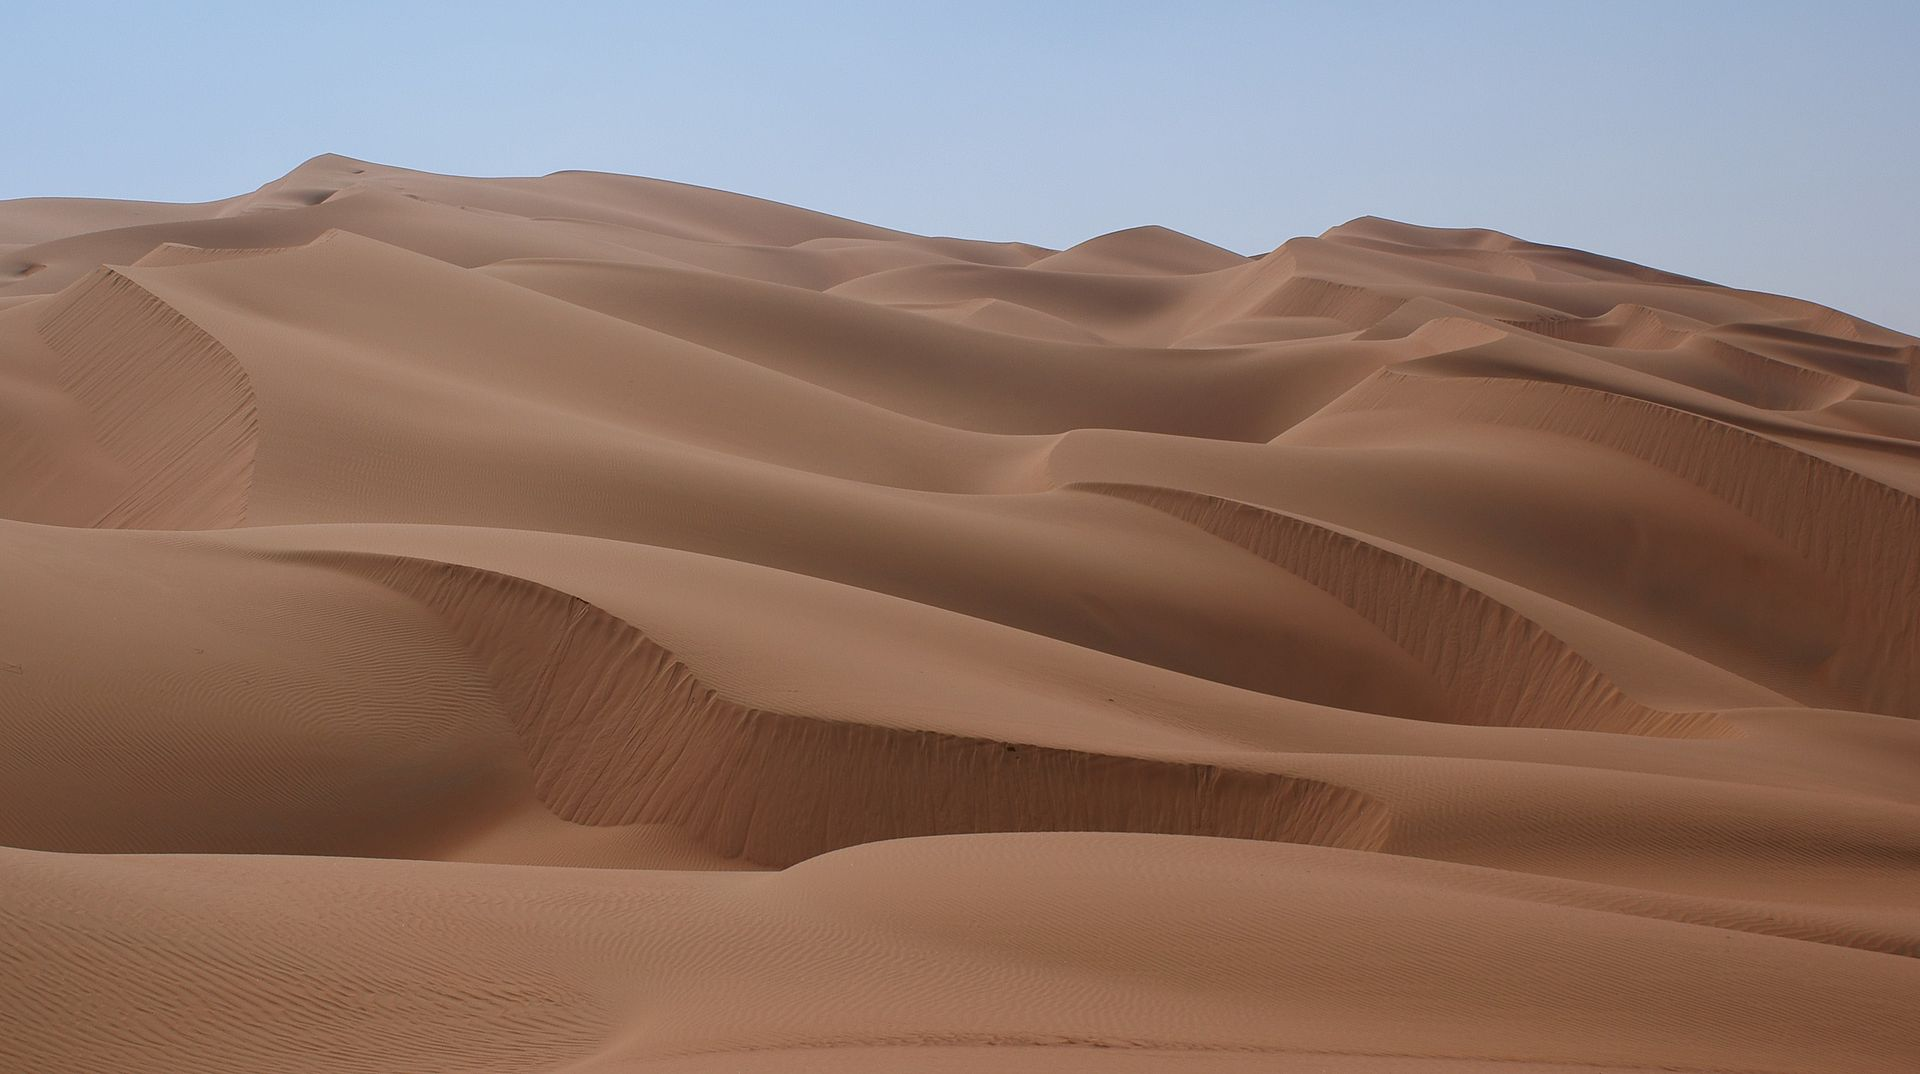
\includegraphics[width=\textwidth]{dunes.jpg}
\end{overlayarea}
\end{column}
\end{columns}
\end{frame}

\begin{frame}
	\frametitle{Multi Armed Bandit (MAB)}
	\begin{columns}
		\begin{column}{.65\textwidth}
			\begin{overlayarea}{\textwidth}{\textheight}
			\vspace{.5cm}
			\begin{itemize}
				\setlength{\itemsep}{20pt}
				\item<1-> Arms $a \in \Aspace$
				\item<2-> Expected payoff $\mu(a)$
				\item<3-> Goal: $\min \Reg(T) = \sum\limits_{t=1}^T[\mu(a^*) - \mu(a_t)]$
				\item<4-> Wide literature on \enb{directed exploration}~\citep{bubeck2012regret,lattimore2019bandit}	
		\end{itemize}
		\end{overlayarea}
		\end{column}
		\begin{column}{.35\textwidth}
			\begin{overlayarea}{\textwidth}{\textheight}
			\vspace{.2\textheight}
			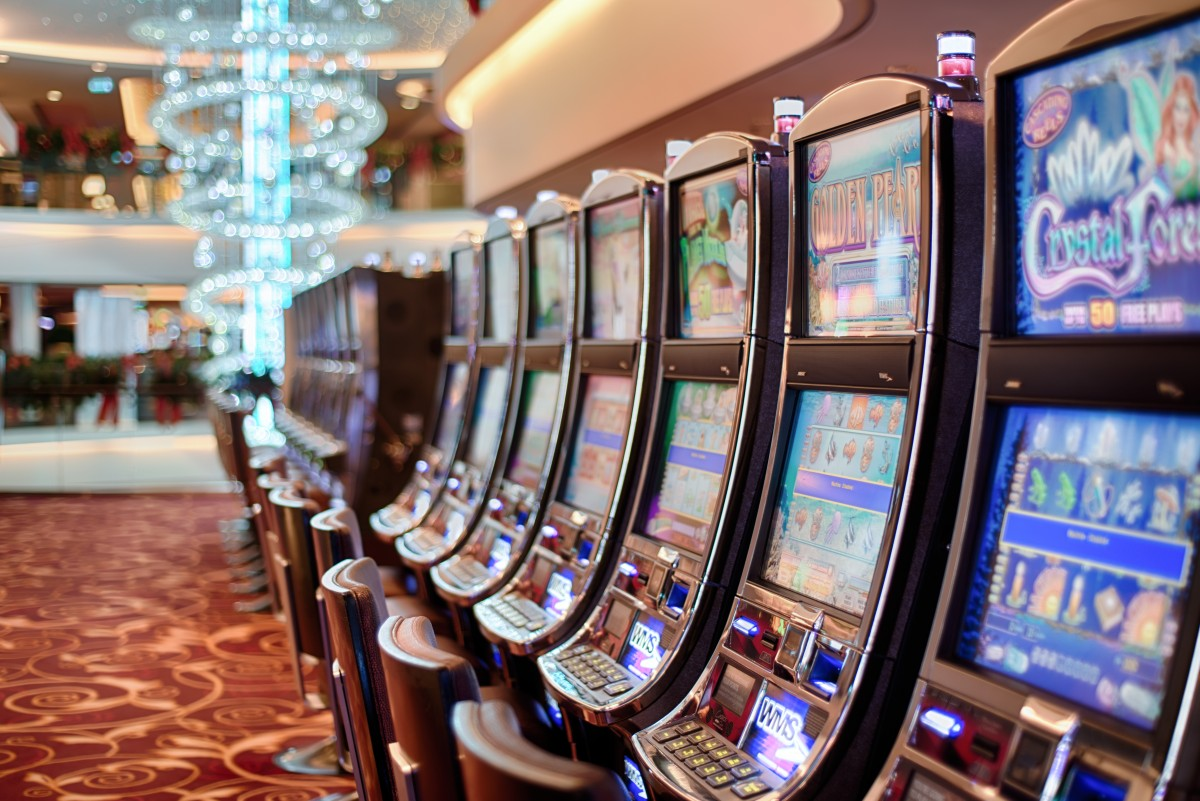
\includegraphics[width=\textwidth]{slot.jpg}
			\end{overlayarea}
	\end{column}
	\end{columns}
\end{frame}

\begin{frame}
\frametitle{Optimism in Face of Uncertainty}
\begin{itemize}
	\item<2-> OFU strategy (\eg UCB~\citep{lai1985asymptotically}):
\end{itemize}
	\[
	a_t\hspace{.5cm} =\hspace{.5cm} \arg\max_{a\in\Aspace}\hspace{.5cm} \underbrace{\vphantom{C\sqrt{\frac{\log(\frac{1}{\delta})}{\#a}}}\widehat{\mu}(a)}_{\textbf{ESTIMATE}} \hspace{.5cm}
	%
	\only<1>{\phantom{+\hspace{.5cm} \underbrace{C\sqrt{\frac{\log(\frac{1}{\delta})}{\#a}}}_{\textbf{EXPLORATION BONUS}}}
	}
	%
	\only<2->{+\hspace{.5cm} \underbrace{C\sqrt{\frac{\log(\frac{1}{\delta})}{\#a}}}_{\textbf{EXPLORATION BONUS}}}
	\]
\vspace{20pt}
\begin{itemize}
	\setlength{\itemsep}{20pt}
	\item<3-> Idea: be \enb{optimistic} about unknown arms
	\item<4-> Can be applied to RL~(\eg~\cite{jaksch2010near})
\end{itemize}
\end{frame}

\begin{frame} 
\frametitle{Policy Optimization as a MAB } 
\begin{columns}
\begin{column}{.65\textwidth}
\begin{overlayarea}{\textwidth}{.75\textheight}
\begin{itemize}
	\setlength{\itemsep}{20pt}
	\item<1-> \enb{Arms:} parameters $\vtheta$\vfill
	\item<2-> \enb{Payoff:} expected return $J(\vtheta)$\vfill
	\item<3-> \eno{Continuous MAB}: we \emph{need} structure~\citep{kleinberg2013bandits}
	\vspace{.5cm}
	\[
		\vtheta_t\hspace{.2cm} =\hspace{.2cm} \arg\max_{\vtheta\in\Theta}\hspace{.5cm} \vphantom{C\sqrt{\frac{\log(\frac{1}{\delta})}{\#a}}}\textcolor{orangep}{\widehat{J}(\vtheta_t)} \hspace{.5cm}+\hspace{.2cm} C\sqrt{\frac{\log(\frac{1}{\delta})}{\textcolor{orangep}{\#\vtheta}}}
	\]
\end{itemize}
\end{overlayarea}
\end{column}
\begin{column}{.65\textwidth}
\begin{overlayarea}{\textwidth}{\textheight}
\only<1>{
	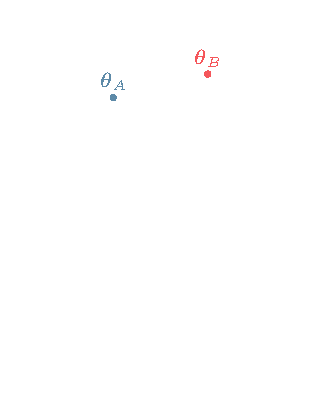
\includegraphics[]{animation/spaces10.pdf}
}
\only<2>{
	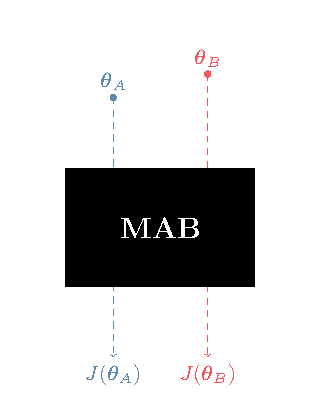
\includegraphics[]{animation/spaces11.pdf}
}
\only<3>{
	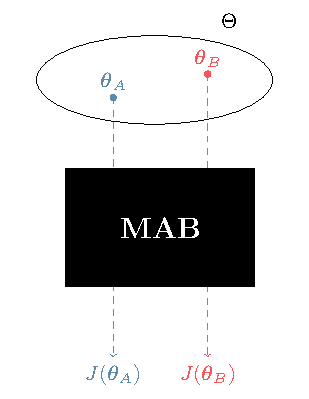
\includegraphics[]{animation/spaces6.pdf}
}
\end{overlayarea}
\end{column}
\end{columns}
\end{frame}

\begin{frame} 
\frametitle{Exploiting Arm Correlation} 
\begin{columns}
	\begin{column}{.45\textwidth}
			\begin{overlayarea}{\textwidth}{\textheight}
			\only<1>{
				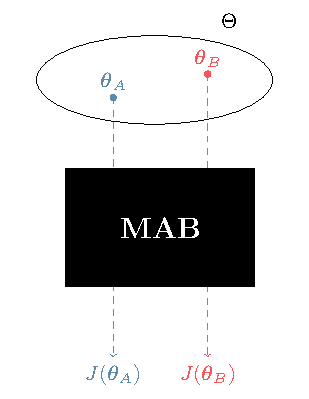
\includegraphics[]{animation/spaces6.pdf}
			}
			\only<2>{
				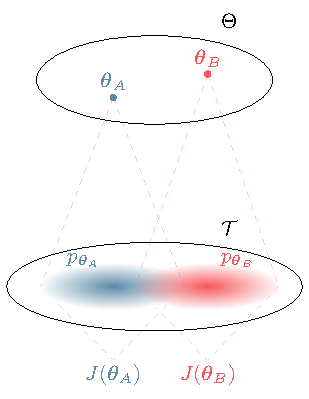
\includegraphics[]{animation/spaces7.pdf}
			}
			\only<3>{
				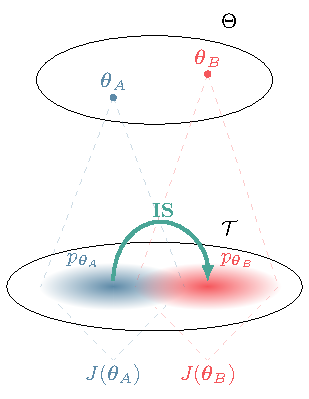
\includegraphics[]{animation/spaces12.pdf}
			}
		\end{overlayarea}
		
	\end{column}
	\begin{column}{.65\textwidth}
	\begin{overlayarea}{\textwidth}{.75\textheight}
		\begin{itemize}
			\setlength{\itemsep}{20pt}
			\item<2-> Arms correlate through overlapping trajectory distributions
			\item<3> Use \textbf{\textcolor{greenp}{Importance Sampling (IS)}} to transfer information
			\vspace{20pt}
			\[
				J(\textcolor{redp}{\vtheta_B}) = \mathop{\mathbb{E}}\limits_{\tau\sim \textcolor{poliblue1}{p_{\vtheta_A}}}\left[
					\frac{\textcolor{redp}{p_{\vtheta_B}}(\tau)}{\textcolor{poliblue1}{p_{\vtheta_A}}(\tau)}R(\tau)
				\right]
			\]
		\end{itemize}
	\end{overlayarea}
	\end{column}
\end{columns}
\end{frame}


\begin{frame} 
\frametitle{The OPTIMIST index~\citep{papini2019optimistic}} 
\begin{overlayarea}{\textwidth}{.5\textheight}
\begin{itemize}
	\setlength{\itemsep}{20pt}
	\item A \enb{UCB-like} index:
	\begin{align*}
	\large
		\vtheta_t \quad = \quad \arg\max_{\vtheta\in\Theta}
		\underbrace{\wc{J}_t(\vtheta)}_{\substack{\textbf{ESTIMATE}\\\\\text{a \enb{robust} \enb{multiple}}\\ \text{ importance sampling estimator}}}
		\only<1>{\phantom{
			+\qquad
			\underbrace{C\,
				\sqrt{\frac{d_{2}(p_{\vtheta}\|\Phi_{t})\log\frac{1}{\delta_t}}{t}}}_{\substack{\textbf{EXPLORATION BONUS}\\\\\text{\enb{distributional} distance} \\ \text{from previous arms}}}}}
		\only<2->{
		+\qquad
		\underbrace{C\,
		\sqrt{\frac{{d_{2}(p_{\vtheta}\|\Phi_{t})}\log\frac{1}{\delta_t}}{t}}}_{\substack{\textbf{EXPLORATION BONUS:}\\\\\text{\enb{distributional} distance} \\ \text{from previous solutions}}}}
	\end{align*}
\end{itemize}
\end{overlayarea}
\vspace{-10pt}
\begin{overlayarea}{\textwidth}{.25\textheight}
\only<1>{
	\hspace{.3\textwidth}
	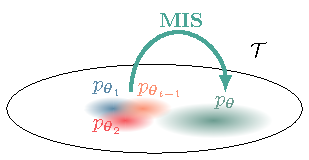
\includegraphics[]{animation/spaces8.pdf}
}
\only<2>{
	\hspace{.3\textwidth}
	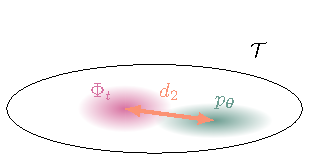
\includegraphics[]{animation/spaces9.pdf}
}
\end{overlayarea}
\end{frame}

\begin{frame}
\frametitle{Robust Multiple Importance Sampling Estimator}
\begin{itemize}
	\setlength{\itemsep}{20pt}
	\item<1-> Use \enb{Multiple} Importance Sampling (MIS)~\citep{veach_optimally_1995} to reuse \emph{all} past experience
	\item<2-> Use \enb{dynamic truncation} to prevent \eno{heavy-tails}~\citep{bubeck2013bandits,metelli2018policy}
\end{itemize}
\begin{overlayarea}{\textwidth}{\textheight}
	\vspace{1.5cm}
	\[
	\only<1>{
		\widehat{J}_t(\vtheta) = \frac{1}{t}\sum_{k=0}^{t-1}\underbrace{\frac{p_{\vtheta}(\tau_k)}{\Phi_t(\tau_k)}}_{\textbf{MIS weight}}R(\tau_k), \qquad \underbrace{\Phi_t(\tau) = \frac{1}{\tau}\sum_{k=0}^{t-1}p_{\vtheta_k}(\tau)}_{\textbf{mixture}}
	}
	\only<2>{
	\wc{J}_t(\vtheta) = \frac{1}{t}\sum_{k=0}^{t-1}{\color{poliblue1}\min\left\{M_t, \frac{p_{\vtheta}(\tau_k)}{\Phi_t(\tau_k)}\right\}}R(\tau_k), \qquad \underbrace{M_t = \sqrt{\frac{td_{2}(p_{\vtheta}\|\Phi_t)}{\log(1/\delta_t)}}}_{\textbf{threshold}}
	}
	\]
\end{overlayarea}
\end{frame}

\begin{frame}
\frametitle{Exploration Bonus}
\begin{itemize}
	\item<1-> Measure novelty with the \emph{exponentiated} \enb{\Renyi 
	divergence}~\citep{cortes2010learning, metelli2018policy}
	\vspace{5pt}
	\[
		d_2(p_{\vtheta}\| \Phi_t) = \int \left(\frac{\de p_{\vtheta}}{\de \Phi_t}\right)^2 \de \Phi_t
	\]
	\vspace{10pt}
	\item<2-> Used to \enb{upper bound} the true value (OFU):
	\vspace{5pt}
	\[
		J(\vtheta)\quad \leq\quad \wc{J}_t(\vtheta)\quad + \quad C\,
		\sqrt{\frac{d_{2}(p_{\vtheta}\|\Phi_{t})\log\frac{1}{\delta_t}}{t}} \qquad \text{with high probability}
	\] 
\end{itemize}
\end{frame}

\begin{frame} 
\frametitle{Sublinear Regret}
\begin{overlayarea}{\textwidth}{.4\textheight}
\begin{itemize}
	\setlength{\itemsep}{20pt}
	\item<1-> $\mathop{Regret}(T) = \sum_{t=0}^T J(\vtheta^*) - J(\vtheta_t)$
	\vfill
	\item<2-> \enb{Compact}, $d$-dimensional parameter space $\Theta$
	\vfill
	\item<3-> Under \enb{mild assumptions} on the policy class, with high probability:
\end{itemize}
\end{overlayarea}
\LARGE
\begin{align*}
\mathop{Regret}(T) = \wt{\mathcal{O}}\left(\sqrt{dT}\right)
\end{align*}
\end{frame}

\begin{frame} 
\frametitle{OPTIMIST in Practice}
\begin{itemize}
	\setlength{\itemsep}{20pt}
	\item<1-> Easy implementation only for \emph{parameter-based exploration}~\cite{sehnke2008policy}
	\item<2-> Difficult index optimization $\implies$ \eno{discretization}
	\item<3-> Computational time can be traded-off with regret
	\vspace{20pt}
	\[
		\wt{\mathcal{O}}\left(dT^{(1-\epsilon/d)}\right) \text{ regret } \implies \mathcal{O}\left(t^{(1+\epsilon)}\right) \text{ time }
	\]
\end{itemize}
\end{frame}

\begin{frame}
\frametitle{Empirical Results} 
\vspace{.5cm}
\begin{columns}
	\begin{column}{.5\textwidth}
		\begin{overlayarea}{\textwidth}{\textheight}
		\centering
		{\bf River Swim}
		\begin{figure}
			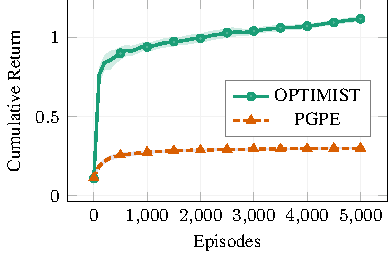
\includegraphics[width=\textwidth]{river.pdf}
		\end{figure}
	\end{overlayarea}	
	\end{column}
\hfill
	\begin{column}{.5\textwidth}
		\begin{overlayarea}{\textwidth}{\textheight}
		\centering
		\only<2->{
		{\bf Mountain Car}
		\begin{figure}
			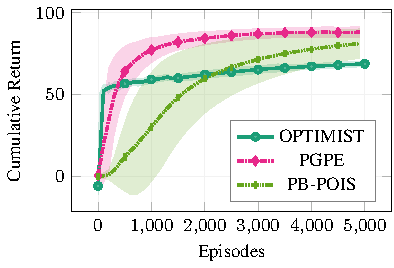
\includegraphics[width=\textwidth]{mc.pdf}
		\end{figure}
	}
	\end{overlayarea}
	\end{column}
\end{columns}
\end{frame}

\begin{frame}
\frametitle{Future Work}
\begin{itemize}
	\setlength{\itemsep}{20pt}
	\item<1-> Extend to action-based exploration
	\item<2-> Improve index optimization
	\item<3-> Posterior sampling~\citep{thompson1933likelihood}
\end{itemize}
\end{frame}


\begin{frame}
\frametitle{The Abstract Problem~\citep{chu2019probability}}
\begin{columns}
	\begin{column}{.65\textwidth}
		\begin{overlayarea}{\textwidth}{\textheight}
			\vspace{1cm}
			\begin{itemize}
			\setlength{\itemsep}{20pt}
			\item<1-> Outcome space $\mathcal{Z}$ 
			\item<2-> Decision set $\mathcal{P}\in\Delta(\mathcal{Z})$
			\item<3-> Payoff $f:\mathcal{Z}\to\Reals$
			\item<4-> $\max\limits_{p\in\mathcal{P}}\mathbb{E}_{z\sim p}\left[f(z)\right]$
		\end{itemize}
		\end{overlayarea}
	\end{column}
	\begin{column}{.35\textwidth}
		\begin{overlayarea}{\textwidth}{\textheight}
			\vspace{.2\textheight}
			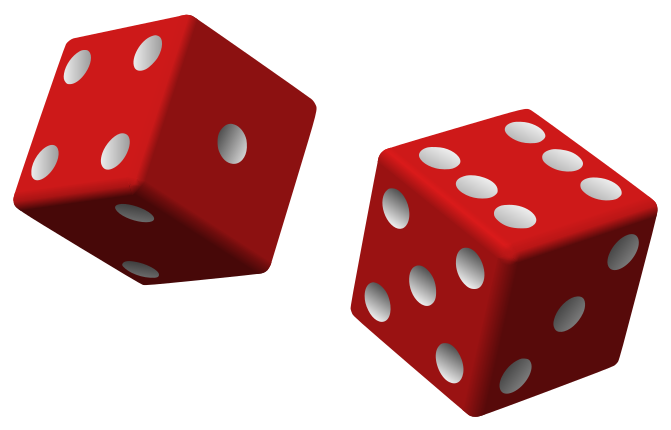
\includegraphics[width=\textwidth]{dice.png}
		\end{overlayarea}
	\end{column}
\end{columns}
\end{frame}

\begin{frame}[plain]
%\frametitle{Thanks} 
\begin{center}
	\huge{\enb{Thank you for your attention!}}
\end{center}
		\vspace{.5cm}
		\emph{Papini, Matteo, Alberto Maria Metelli, Lorenzo Lupo, and Marcello Restelli. "Optimistic Policy Optimization via Multiple Importance Sampling." In International Conference on Machine Learning, pp. 4989-4999. 2019.}
		\vspace{.5cm}
		\begin{columns}
			\begin{column}{.75\textwidth}
			\begin{itemize}
				\setlength{\itemsep}{20pt}
				\item[] Code: \url{github.com/WolfLo/optimist}
				\item[] Contact: matteo.papini@polimi.it
				\item[] Web page: \url{t3p.github.io/icml19} 
			\end{itemize}	
			\end{column}
			\begin{column}{.25\textwidth}
				
\includegraphics[width=\textwidth]{qr.png} 
			\end{column}
		\end{columns}
\end{frame}


%%%%%%%%%%%%%%%%%%%%%%%%%%%%%%%%%%%%%%%%%%%%%%%%%%%%%%%%%%%%%%%%%%%%%%%%%%%%%%%%%%%%%%%%%
\begin{frame}[allowframebreaks,fragile]
\frametitle{References}
\bibliographystyle{plainnat}
\bibliography{../biblio.bib}
\end{frame}
%%%%%%%%%%%%%%%%%%%%%%%%%%%%%%%%%%%%%%%%%%%%%%%%%%%%%%%%%%%%%%%%%%%%%%%%%%%%%%%%%%%%%%%%%

%%Backup Slides


\end{document}
